\chapter{Analysis Models}
\label{chap:AM}

This chapter provides a general overview of the main concepts gathered during
the analysis phase, in particular those concerning the software system types
(i.e. classes, datatypes, and enumerations), as well as the actors that interact
with the software system through their interfaces. Figures included in the
Messir Requirement Document that correspond to the  the \glspl{Concept Model} and the \glspl{Environment
Model} could be also included in this chapter, as a means of synthesizing what
are the requirements to which the design is supposed to sketch a solution.




\section{Concept Model}

%\usepackage{graphics} is needed for \includegraphics
\begin{figure}[H]
\begin{center}
  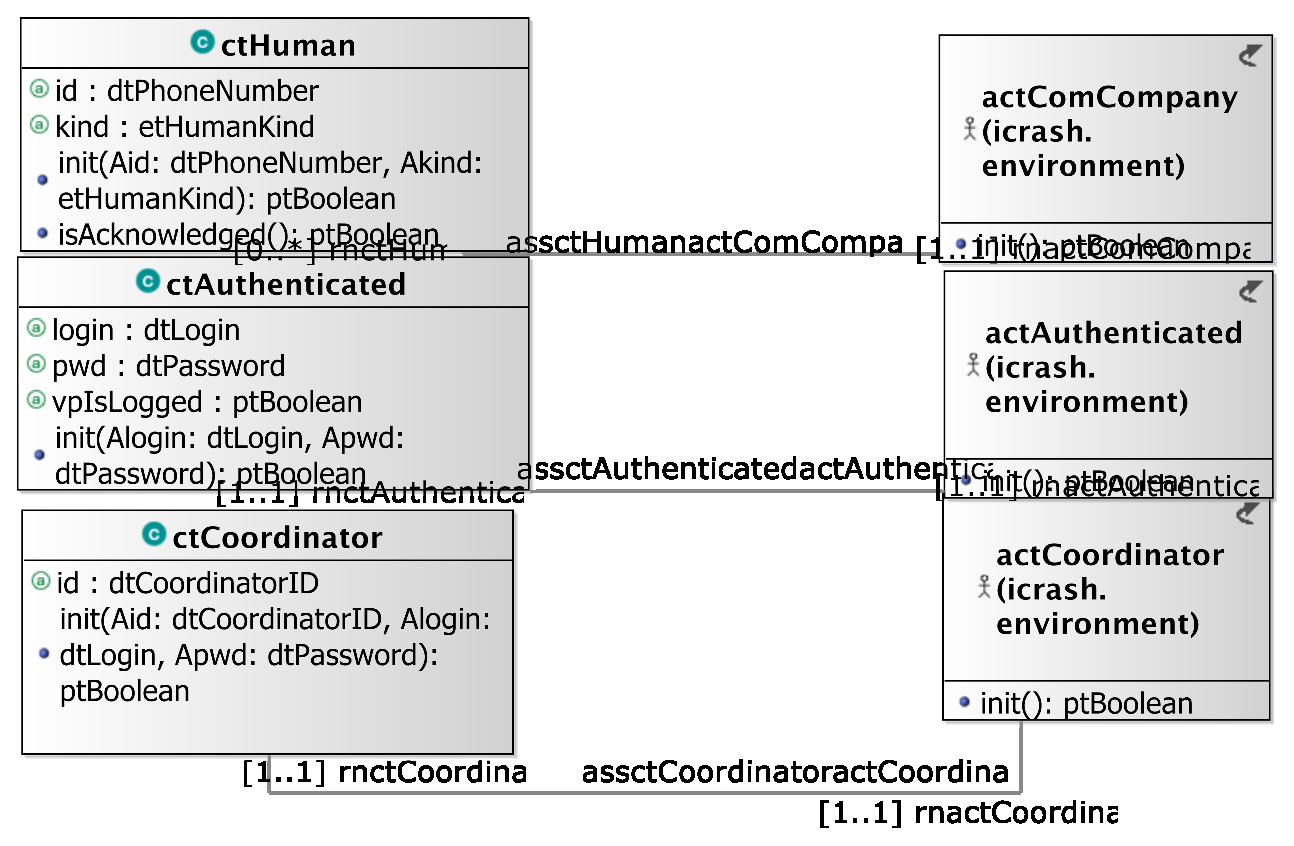
\includegraphics[width=400px]{images/analysis/concept-model/global/PrimaryTypes-Classes/01/cm-pt-ct-gv-01.eps}
  \caption{Concept Model - Primary types class types global view}
  \label{figureLabel}
\end{center}
\end{figure}

\subsection{Primary types - Class types descriptions}

\subsubsection{ctAuthenticated}
Used to model system’s representation about actors that need to authenticate to
access some specific functionalities.

\subsubsection{ctAdministrator}
Used to caracterize internally the entity that is responsible of administrating
the \mysystemname system.

\subsubsection{ctCoordinator}
Used to model system’s representation about the actors that have
the responsibility to handle alerts and crisis.

\subsubsection{ctCrisis} 
Used to model crisis that are infered from the reception of at least
one alert message. Crisis aer entities that are handled by the \mysystemname system.

\subsubsection{ctHuman} 
Used to model system’s representation about the indirect actors that has
alerted of potential crisis.

\subsubsection{ctAlert}
Used to model crisis alerts sent by any human having communication capability
using communication companies belonging to the system’s environment.

\subsubsection{ctState} 
Used to model the system. There is only one instance at any state of the
abstract machine after creation.

\subsection{Primary types - Datatypes types descriptions}

\subsubsection{Datatypes}

\paragraph*{\textbf{dtAlertID}}
A string used to identify alerts.

\paragraph*{\textbf{dtComment}}
A datatype made of a string value used to receive,store and send
textual information about crisis and alerts.

\paragraph*{\textbf{dtCoordinatorID}}
A string used to identify coordinators.

\paragraph*{\textbf{dtCrisisID}}
A string used to identify crisis.

\paragraph*{\textbf{dtGPSLocation}}
Used to define coordinates of geograpical positions on earth. It
is defined a couple made of a latitude and a longitude.

\paragraph*{\textbf{dtLatitude}}
Used to define a latitude value of a geograpical positions on earth.

\paragraph*{\textbf{dtLogin}}
A login string used to authentify an \mysystemname user

\paragraph*{\textbf{dtLongitude}}
Used to define a longitude value of a geograpical positions on
earth.

\paragraph*{\textbf{dtPassword}}
A password string used to authentify an \mysystemname user

\paragraph*{\textbf{dtPhoneNumber}}
A string used to store the phone number from the human declaring
the crisis or the alert.

\subsubsection{Enumerations}

\paragraph*{\textbf{etAlertStatus}} 
This type is used to indicate the different validation status of
an alert.

\paragraph*{\textbf{etCrisisStatus}} 
This type is used to indicate the different handling status of a
crisis.

\paragraph*{\textbf{etCrisisType}} 
This type is used to indicate the different types of a crisis.

\paragraph*{\textbf{etHumanKind}} 
This type is used to indicate the kind of human that informs about a
car crash crisis.

\subsection{Secondary types - Datatypes types descriptions}

\subsubsection{Datatypes}

\paragraph*{\textbf{dtSMS}}
A datatype made of a string value used to send textual information to human
mobile devices.

% \begin{figure}
% \begin{center}
% \includegraphics[width=\textwidth]{./images/myfigure.eps}
% \end{center}
% \caption{Caption for my figure}
% \label{fig:myfigure}
% \end{figure} 


   

\section{Environment Model}

%\usepackage{graphics} is needed for \includegraphics
\begin{figure}[H]
\begin{center}
  \includegraphics[width=400px]{images/analysis/environment-model/global/01/em-gv-01.eps}
  \caption{Environment Model - Global View}
  \label{env-global}
\end{center}
\end{figure}

\subsection{actMsrCreator Actor}
Represents the creator stakeholder in charge of state and environment
initialization.

\subsection{actActivator Actor}
Represents a logical actor for time automatic message sending based on system’s
or environment status.

\subsection{actAuthenticated Actor}
Abstract actor providing reusable input and output interfaces for actors that
need to authenticate themselves.

\subsection{actAdministrator Actor}
Represents an actor responsible of administration tasks for the \mysystemname
system. 

\subsection{actCoordinator Actor}
Represents actor responsible of handling one or several crisis for the
\mysystemname system.

\subsection{actComCompany Actor}
Represents the communication company stakeholder ensuring the input/ouput of
textual messages with humans having communication devices.
